\section{Reconhecimento Facial}

O reconhecimento facial é uma das atividades mais comuns realizadas diariamente por seres vivos dotados de certa inteligência. Essa simples atividade vem despertando o interesse de pesquisadores que trabalham com Visão Computacional e Inteligência Artificial. O objetivo desses pesquisadores é de construir sistemas artificiais capazes de realizar o reconhecimento de faces humanas e a partir desta capacidade construir os mais diferentes tipos de aplicações: sistemas de vigilância, controles de acesso, definções automáticas de perfis, entre outros \cite{oliveira}.

No anos 70, os estudos do reconhecimento facial eram baseados sobre atributos faciais mensuráveis como olhos, nariz, sobrancelhas, bocas, entre outros. Porém, os recursos computacionais eram escassos e os algoritmos de extração de características eram ineficiêntes. Nos anos 90, as pesquisas na área ressurgiram, inovando os métodos existentes \cite{hong, saocarlos} e disseminando a técnica.

Um dos motivos que incentivou os diversos estudos sobre reconhecimento facial são as vantagens que o mesmo possui em relação a impressão digital e a íris.  No reconhecimento por impressão digital, a desvantagem consiste no fato que nem todas as pessoas possuem uma impressão digital com ``qualidade'' suficiente para ser reconhecida por um sistema. Já o reconhecimento por íris apresenta uma alta confiabilidade e larga variação, sendo estável pela vida toda. Porém, a desvantagem está relacionada ao modo de captura da íris que necessita de um alinhamento entre a câmera e os olhos da pessoa \cite{saocarlos}. 

Basicamente existem duas particularidades que fazem da face uma característica biométrica bastante atrativa \cite{drovetto}:

	\begin{enumerate}
		\item A aquisição da face é feita de forma fácil e não-intrusiva;
		\item Possui uma baixa privacidade de informação: como a face é exposta constantemente, caso uma base de faces seja roubada, essas informações não representam algum risco e não possibilitam um uso impróprio;
	\end{enumerate}

Umas das maiores dificuldades dos sistemas de reconhecimento é tratar a complexidade dos padrões visuais. Mesmo sabendo que todas as faces possuem padrões reconhecidos, como boca, olhos e nariz, elas também possuem variações únicas que devem ser utilizadas para determinar as características relevantes. Outra dificuldade encontrada em relação a essas características é que elas possuem uma larga variação estatística para serem consideradas únicas para cada indivíduo. O ideal seria que a variância inter-classe seja grande e a intra-classe pequena, pois assim imagens de diferentes faces geram os códigos mais diferentes possíveis, enquanto imagens de uma mesma face geram os códigos mais similares possíveis. Portanto, estabelecer uma representação que capture as características ideias é um difícil problema \cite{saocarlos}.

Do ponto de vista geral, o recohecimento facial continua sendo um problema aberto por causa de várias dificuldades que aumentam a variância intra-classe \cite{hong}. Entre estas, destacamos as mais comuns \cite{saocarlos}:

	\begin{itemize}
		\item iluminação;
		\item ângulos e poses;
		\item expressões;
		\item comésticos e acessórios;
		\item extração da face do contexto ou do fundo;
	\end{itemize}

No contexto de identificação, o reconhecimento facial se resume no reconhecimento de um ``retrato'' frontal, estático e controlado. Estático pois os ``retratos'' utilizados nada mais são que imagens, podendo ser tanto de intensidade quanto de profunidade e controlado pois a iluminação, o fundo, a resolução dos dispositivos de aquisição e a distância entre eles e as faces são essencialmente fixas durante o processo de aquisição da imagem \cite{hong}.

Basicamente, o processo de reconhecimento facial pode ser divido em duas tarefas principais \cite{hong}:

	\begin{enumerate}
		\item Detecção de faces em imagens;
		\item Reconhecimento das faces encontradas;
	\end{enumerate}

Falaremos dessas duas tarefas separadamente nas próximas subseções.

% ################################################################################################################################

\subsection{Detecção de Faces em imagens}
	
A primeira etapa para o reconhecimento de faces é a detecção de um rosto, e a partir daí a comparação do mesmo com modelos conhecidos pelo sistema \cite{hong, oliveira}. Em um sistema de reconhecimento facial, tanto o tempo de resposta quanto a confiabilidade desta etapa influênciam diretamente no desempenho e o emprego deste sistema \cite{oliveira}.

A detecção de faces é definida como o processo que determina a existência ou não de faces em uma imagem e uma vez encontrada alguma face, sua localização deve ser apontada através de um enquadramento ou através de suas coordenadas dentro da imagem \cite{oliveira}. A Figura \ref{enquadramentoRosto} representa um exemplo da detecção de uma face em uma imagem.

	\begin{figure}[hbt]
		\begin{center}
			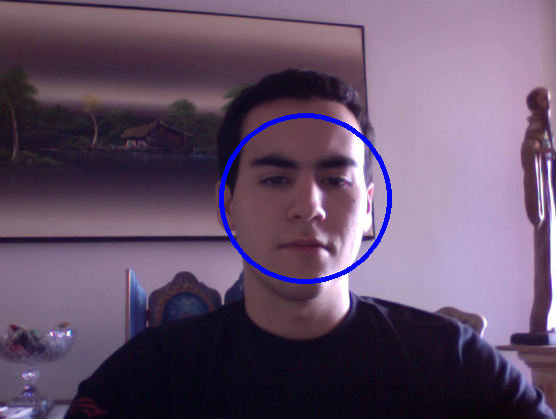
\includegraphics[height=9.5cm,width=12.5cm]{figuras/2.FundamentacaoTeorica/enquadramentoRosto.png}
		\end{center}
		\caption{Exemplo de um processo de detecção de uma face em uma imagem.}
		\label{enquadramentoRosto}
	\end{figure}

O processo de detecção de faces geralmente é dificultado pelas seguintes razões mostradas a seguir:

	\begin{enumerate}
		\item \textbf{Pose}: as imagens de uma face podem variar de acordo com a posição relativa entre a camêra e a face (frontal, 45 graus, perfil, ``de cabeça para baixo''), e com isso algumas características da face, como olhos e nariz, podem ficar parcialmente ou totalmente ocultadas \cite{yang}.
		\item \textbf{Presença de acessórios}: características faciais básicas importantes para o processo de detecção podem ficar ocultadas pela presença de acessórios, como óculos, bigode, barba, entre outros \cite{oliveira, yang}. 
		\item \textbf{Expressões faciais}: embora a maioria das faces apresente estruturas semelhantes (olhos, bocas, nariz, entre outros) e são dispostas aproximadamente na mesma configuração de espaço, pode haver um grande número de componentes não rigídos e texturas diferentes entre as faces. Um exemplo são as flexibilizações causadas pelas expressões faciais~\cite{oliveira, yang};
		\item \textbf{Obstrução}: faces podem ser obstruídas por outros objetos. Em uma imagem com várias faces, uma face pode obstruir outra \cite{yang}.
		\item \textbf{Condições da imagem}: a não previsibilidade das condições da imagem em ambientes sem restrições de ilimuniação, cores e objetos de fundo \cite{oliveira, yang}.
	\end{enumerate}

Atualmente, já existem diferentes métodos/técnicas de detecção de faces. Tais métodos podem ser baseados em imagens de intensidade e de cor ou em imanges 3D. Focaremos nos principais métodos de imagens de cor e de intensidade que serão utilizados neste trabalho. Estes podem ser divididos em 4 categorias:

	\begin{enumerate}
		\item \textbf{Métodos baseados em Conhecimento:} métodos, desenvolvidos principalmente para localização facial, beaseados em regras derivadas do conhecimento dos pesquisadores do que constitui uma típica face humana. Normalmente, captura as relações existentes entre as características faciais. É fácil econtrar regras que descrevem as caracterísicas faciais. Por exemplo, uma face sempre é constituída por dois olhos simétricos, um nariz e uma boca. As relações entre essas características podem ser representadas pelas distâncias relativas e posições. Este método possui desvantagens em relação a construção do conjunto de regras. Se estas são muito gerais, corre-se o risco de que o sistema que as utiliza apresentar uma alta taxa de falsos positivos. Se são muito específicas podem ser ineficazes ao tentar detectar faces por não satisfizerem todas as regras, diminuindo muito a precisão da detecção~\cite{yang,lopes};

		\item \textbf{Métodos baseados em Características Invariantes:} esses algoritmos tem como objetivo principal encontrar as características estruturais que existem mesmo quando a postura, ``ponto de vista'', condições de iluminação variam. E por meio dessas características localizar a face. São desenvolvidos principalmente para localização facial \cite{yang}. A principal desvantagem desse método é que tais características invariantes podem ser corrompidas devido a condições de ilumincação ou algum tipo de ruído, comprometendo a eficiência. A cor da pele e a textura da face são as principais características invariantes que podem ser utilizadas para separar a face de outros objetos~\cite{lopes};

		\item \textbf{Métodos baseados em Templates:} vários padrões comuns de um rosto são armazenados tanto para descrever o rosto como um todo quanto para descrever as características faciais separadamente. As correlações entre as imagens de entrada e os padrões armazenados são comuptados para detecção. Esses métodos são desenvolvidos para serem utlizados como localização e detecção facial~\cite{yang};

		\item \textbf{Métodos baseados em Aparência:} recebem este nome devido ao fato de não utilizarem nenhum conhecimento a priori sobre o objeto ou características a serem detectadas. Em contraste com os métodos baseado em templates, os modelos são retirados de um conjunto de imagens de treinamento que devem capturar a variabilidade da face. Esses modelos retirados são utilizados para detecção. Nesta classe de algoritmos surge os conceitos de aprendizado e treinamento, uma vez que as informações necessárias para realizar a tarefa de detecção são retiradas do próprio conjunto de imagens sem intervenção externa. São métodos desenvolvidos principalmente para detecção de faces~\cite{yang, lopes};

	\end{enumerate}

Um problema relacionado e muito importante é como avaliar a performance dos métodos de detecção de faces propostos. Para isso, muitas métricas foram adotadas como tempo de aprendizagem, número de amostras necessárias no treinamento e a proporção entre taxas de detecção e ``falso alarme''. Esta última é dificultada pelas diferentes definições para as taxas de detecção e falso alarme adotadas pelos pesquisadores~\cite{yang}.

O método que será utilizado nesse trabalho será o método \textit{Viola-Jones}}. Este é um  método para detecção de objetos que minimiza o tempo de computação e possui uma alta acurácia permindo detecção de faces em tempo real. Esse método pode ser utilizado para construir uma abordagem de detecção facial rápida e eficaz~\cite{violajones}. É o método utilizado na biblioteca \textit{OpenCV}(Open Source Computer Vision) e muito utilizado autalmente.
	
O Método \textit{Viola-Jones} para detecção facial utiliza quatro conceitos chaves~\cite{servodetection,violajones}:
	
	\begin{enumerate}
		\item \textbf{\textit{Haar features}:} simples características retangulares;
		\item \textbf{\textit{Integral Image}:} uma nova representação da imagem que permite uma rápida avaliação de recursos e caracterísitcas;
		\item \textbf{O método \textit{AdaBoost}}: um método de aprendizagem de máquina utilizado para construir um classificador,  selecionando um pequeno número de características importantes usando \textit{AdaBoost};
		\item \textbf{Classificador em Cascata}: classificador que combina muitas características de maneira eficiente;
	\end{enumerate}

	\begin{figure}[hbt]
		\begin{center}
			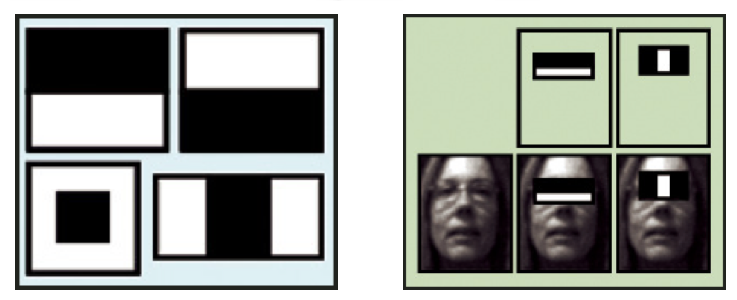
\includegraphics[height=6.5cm,width=12.5cm]{figuras/2.FundamentacaoTeorica/haar_features.png}
		\end{center}
		\caption{Exemplo de simples características retangulares (\texit{Haar Features}). Adaptada de \cite{servodetection}.}
		\label{haarfeatures}
	\end{figure}

A detecção facial em imagens é baseado em simples caracteríticas retangulares (\textit{Haar features}), exemplificada na Figura \ref{haarfeatures}. Existem vários motivos para se usar essas características ao invés de usar diretamente os pixels da imagem. Uma das principais é que sistemas baseados em características são muito mais rápidos que sistemas baseados em pixels~\cite{violajones}. 

\begin{figure}[hbt]
		\begin{center}
			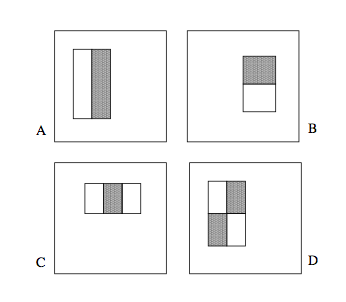
\includegraphics[height=6.5cm,width=12.5cm]{figuras/2.FundamentacaoTeorica/haarfeaturestypes.png}
		\end{center}
		\caption{\texit{Haar Features} com dois, três e quatro retângulos~\cite{violajones}.}
		\label{haarfeaturestypes}
	\end{figure}

Tais simples características são remanecentes das funções de base \textit{Haar}. O método utiliza três tipos de características, exemplificadas na Figura \ref{haarfeaturestypes}: características com dois, três ou quatro retângulos~\cite{violajones}. A presença de uma característica em uma imagem é determinada pela subtração da média dos valores dos pixels da região escura pela média dos valores dos pixels da região clara. Caso o valor seja maior que um limiar, então essa característica é tida como presente~\cite{servodetection}.

O Método \textit{Viola-Jones} não trabalha diretamente com as intensidades da imagem. Para determinar a presença ou ausência de centenas de \textit{Haar features} em cada posição de imagem e em várias escalas de forma eficiente, utiliza uma técnica chamada \textit{Integral Image}. Basicamente, o método consiste em acrescentar pequenas unidades juntas. Neste caso, pequenas unidades são valores de pixels. O valor ``integral'' para cada pixel é a soma de todos os pixels acima e a esquerda. Começando pelo canto superior esquerdo da imagem e atravessando para direita e para baixo, toda a imagem pode ser ``integrada'' com poucas operações por pixels~\cite{servodetection, violajones}. Com a nova representação de imagem criada, qualquer \textit{Haar Feature} pode ser computada para qualquer escala e localização em um tempo constante~\cite{violajones}.

	\begin{figure}[hbt]
		\begin{center}
			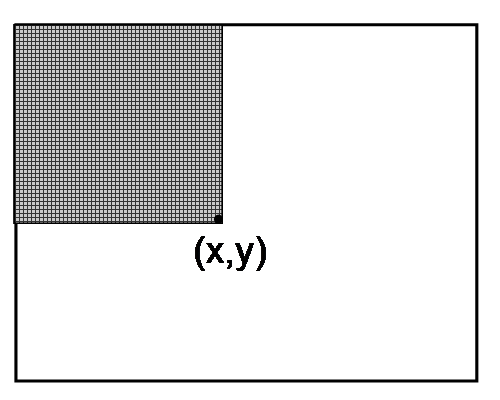
\includegraphics[height=6.5cm,width=12.5cm]{figuras/2.FundamentacaoTeorica/integral_image.png}
		\end{center}
		\caption{Exemplo da aplicação da técnica \texit{Integral Image}. Após a ``integração'' o pixel $\displaystyle (x,y)$ contém a soma dos valores dos pixels do retângulo sombreado. Adaptada de~\cite{servodetection}.}
		\label{integralimage}
	\end{figure}

Na Figura \ref{integralimage}, após a ``integração'', o pixel $\displaystyle (x,y)$ contém a soma de todos os valores de pixels dentro da região retangular sombreada no canto superior esquerdo de $\displaystyle (x,y)$. Para calcular a média dos valores de pixel neste retângulo, basta dividir o valor em $\displaystyle (x,y)$ pela área do retângulo~\cite{servodetection}.

	\begin{figure}[hbt]
		\begin{center}
			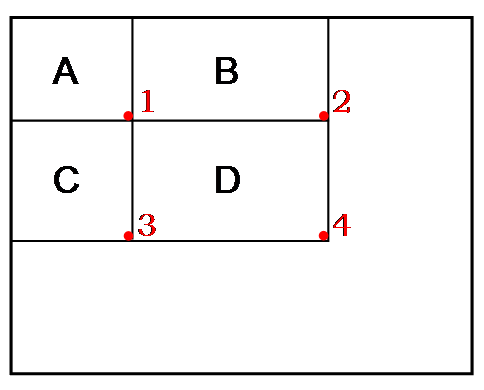
\includegraphics[height=6.5cm,width=12.5cm]{figuras/2.FundamentacaoTeorica/integral_image2.png}
		\end{center}
		\caption{Exemplo utlizado para mostrar como calcular a soma dos valores de pixel de um retângulo que não está localizado no canto superior esquerdo da imagem utilizando \textit{Integral Image}. Adaptado de~\cite{servodetection}.}
		\label{integralimage2}
	\end{figure}

A Figura \ref{integralimage2} mostra como calcular os valores de um retângulo que não está localizado no canto superior esquerdo da imagem. Suponha que se deseja obter a soma dos valores do retângulo em $\displaystyle D$. De maneira intuitiva, pode-se realizar esse cálculo somando os valores dos pixels no retângulo formado por $\displaystyle A+B+C+D$, menos a soma nos retângulos $\displaystyle A+B$ e $\displaystyle A+C$, mais a soma dos valores de pixel em $\displaystyle A$. Em outras palavra, $\displaystyle D = A+B+C+D-(A+B)-(A+C)+A$~\cite{servodetection, violajones}.

Porém, usando \textit{Integral Image}, $\displaystyle A+B+C+D$ é o valor do ponto $\displaystyle 4$, $\displaystyle A+B$ é o valor do ponto $\displaystyle 2$, $\displaystyle A+C$ é o valor do ponto $\displaystyle 3$, e $\displaystyle A$ é o valor do ponto $\displaystyle 1$. Então, com \textit{Integral Image}, você pode obter a soma dos valores de pixel de qualquer retângulo na imagem original usando somente três operações~\cite{servodetection, violajones}:

	\begin{equation}
		(x_4,y_4) - (x_2,y_2) - (x_3,y_3) + (x_1,y_1)
		\label{equacaointegralimage}
	\end{equation} 

Para selecionar os \textit{Haar features} que serão utilizados e para definir os limiares, o método \textit{Viola-Jones} utiliza um método de aprendizagem de máquina chamado \textit{AdaBoost}. Este combina vários classificardores ``fracos'' para criar um classificador ``forte''. 

Um classificador fraco é aquele que só obtém a resposta correta um pouco mais frequente que um ``palpite aleatório''. A combinação desses classficadores ``fracos'', onde cada um ``empurra'' a resposta final um pouco na direção certa, pode ser considerado como um classificador ``forte''. O método \texit{AdaBoost} seleciona um conjunto de classificadores ``fracos'' para combinar e atribui pesos a cada um. Essa combinação ponderada resulta em um classificador ``forte''~\cite{servodetection}.

Em qualquer região de uma imagem, o número total de \textit{Haar features} é muito grande, muito maior que o número de pixels. Para assegurar uma classficação rápida, o processo de aprendizagem deve excluir o maior número de características disponíveis, e focar nas que são críticas. A seleção dessas características é alcançada através de uma simples modificação no método \textit{AdaBoost}: o mecanismo de aprendizagem é construído de forma que cada classificador ``fraco'' retornado dependa de somente uma única característica. Como resultado, cada estágio do processo seleciona um novo classificador ``fraco'' o que pode ser visto como um processo de seleção de características. \textit{AdaBoost} fornece um algoritmo de aprendizagem eficaz~\cite{violajones}.

	\begin{figure}[htb]
		\begin{center}
			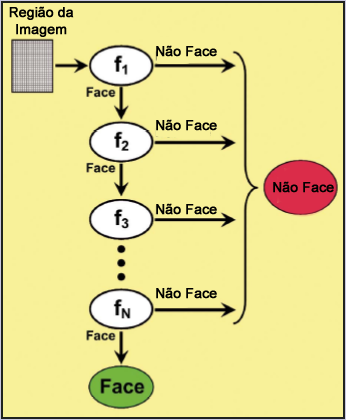
\includegraphics[height=10cm,width=7.5cm]{figuras/2.FundamentacaoTeorica/filterchain.png}
		\end{center}
		\caption{Ilustração de uma classificador em cascata composto com uma cadeia de filtros~\cite{servodetection}.}
		\label{filterchain}
	\end{figure}

O método \textit{Viola-Jones} combina uma série de classificadores \textit{AdaBoost} na forma de uma cadeia de filtros, como na Figura \ref{filterchain}, que recebe o nome de Classificadores em Cascata. Cada filtro em si é um classificador \textit{AdaBoost} com um número relativamente pequeno de classificadores ``fracos''~\cite{servodetection}. 

O limiar de aceitação em cada nível é definido ``baixo'' o suficiente para que passe por todos, ou quase todos, os exemplos de face do conjunto de treinamento (um grande banco de imagens contendo faces). Os filtros em cada nível são treinados para classificar imagens de treinamento que passaram por todas fases anteriores~\cite{servodetection}.

Durante a utilização, se alguma região de uma imagem falhar em passar em um desses filtros, esta é imediatamente classificada como ``não face''. Quando uma região de uma imagem passa por um filtro, ela vai para o próximo filtro na cadeia. As regiões das imagens que passarem por todos os filtros na cadeia são classificadas como ``faces''~\cite{servodetection}.

O algoritmo utilizado para construção dos Classificadores em Cascata alcança um ótimo desempenho e, ao mesmo tempo, reduz drasticamente o tempo de computação. O aspecto chave é que os menores classificadores (filtros), e por isso mais eficientes, podem ser utilizados para rejeitar a maioria das regiões das imagens que não são faces antes que os classifcadores mais complexos sejam utilizados~\cite{violajones}. A ordem dos filtros no classificador é baseado nos pesos que o método \textit{AdaBoost} define para cada filtro. Os filtros com maior peso são colocados no início, para eliminar as regiões das imagens que não são faces o mais rápido possível~\cite{servodetection}. 

O método \textit{Viola-Jones} é adequado para utilização em sistemas de detecção de faces em tempo real. Agora, o próximo passo para o processo de Reconhecimento Facial é comparar as faces encontradas com modelos conhecidos com o sistema para realizar a identificação, o que será mostrado na próxima subseção.

% ################################################################################################################################
% ################################################################################################################################
% ################################################################################################################################

\subsection{Reconhecimento das Faces encontradas}

Na etapa de reconhecimento, as faces detectadas e processadas, serão comparadas com um banco de dados de faces conhecidas. Essa comparação tem uma acurácia média de 30-90\% entre as diversas técnicas. Esse é um forte campo de pesquisa desde a década de 90 e as técnicas se invovam ano ápos ano.

Existem duas variações principais entre as técnicas, as que usam como entrada dados imagens 2D (imagens de intensidade e cor) e as que usam como entradas dados imagens 3D (\textit{depth images}).
As principais técnicas 2D são:
	\begin{enumerate}
		\item \textbf{\textit{Eigenfaces}}
		\item \textbf{Redes Neurais}
		\item \textbf{\textit{Fisher Faces}}
	\end{enumerate}

% Com o surgimento da tecnologia 3D o reconhecimento facial se trasformou mais confiável pois a imagem 3D evita problemas comum em reconhecimentos faciais 2D como a mudança na iluminação, diferentes expressões faciais, maquiagem e orientação da cabeça.
% Algumas técnicas 3D são:
% 	\begin{enumerate}
% 		\item \textbf{``Face Recognition Homepage''}
% 		\item \textbf{``3D Face Recognition''}
% 		\item \textbf{``Active Appearance Models''}
% 	\end{enumerate}

De todos os métodos apresentados o \textit{Eigenfaces} se mostrou de melhor custo benefício, devido ao seu baixo custo computacional e a sua, relativamente alta, confiabilidade.

Este é um algoritmo simples e fácil de implementar e os passos utilizados por ele também são utilizados em muitos métodos avançados. Os princípios básicos por trás dele, como PCA (\textit{Principal Component Analisys} - Analíse de componente principal) e \textit{Distance-Based Matching} (Correspondência Baseada na Distância) aparecem cada vez mais na computação visual e em diversas aplicações de inteligencia artificial \cite{hewitt}.
O \textit{Eigenfaces} trabalha de forma simples, dada uma imagem de um rosto desconhecido e imagens do rosto das pessoas conhecidas executa as seguintes ações \cite{hewitt}:
	\begin{enumerate}
		\item Computa a distância entre a nova imagem e cada uma das imagens já conhecidas.
		\item Seleciona a imagem mais proxima do novo rosto.
		\item Se a distância da nova imagem para a imagem já catalogada for menor que o limite predefinido, ``reconhece'' a imagem caso contrário classifica como ``desconhecida''.
	\end{enumerate}

A distância entre as imagens é medida ponto a ponto. Esta é também chamado de distância euclidiana. A distância euclidiana em duas dimensões entre os pontos $P_1$ e $P_2$ é dada pela fórmula $\displaystyle d_{12} = \sqrt(d_{x2} + d_{y2})$, onde $\displaystyle d_x = x_2 - x_1$ e $\displaystyle d_y = y_2-y_1$ e representada na Figura \ref{distanciaEntrePontos} \cite{hewitt}.

    \begin{figure}[hbt]
		\begin{center}
			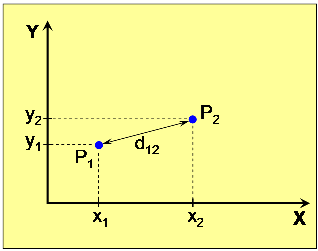
\includegraphics[height=9.5cm,width=12.5cm]{figuras/2.FundamentacaoTeorica/graficoDistanciaEntrePontos.png}
		\end{center}
		\caption{Distância Euclidiana entre dois pontos em duas dimensões \cite{hewitt}.}
		\label{distanciaEntrePontos}
	\end{figure}


Imagens possuem ``ruídos'' e vamos definir ruído como qualquer coisa que atrapalhe na identificação, como por exemplo as diferenças na luminosidade. Cada pixel possui uma intensidade de ruído diferente. Com cada pixel contribuindo para o ruído total, este dificulta o processo de encontrar a imagem correta referente a imagem testada. Uma solução é diminuir a dimensionalidade da imagem tornando assim o ruído menor e sendo possível extrair da imagem as informações importantes \cite{hewitt}.

Um dos métodos existentes para reduzir a dimesionalidade da imagem é o ``PCA - Principal Components Analysis'' \cite{hewitt}.

Para se ter uma idéia do que é o PCA, vejamos um caso especial chamado de \textit{least squares line fit}. O lado esquerdo da Figura \ref{exemploPCA} mostra um exemplo de uma linha média entre três pontos, que são, no mapa em 2D, Los Angeles, Chicago e Nova York. Estes três pontos do mapa são quase, mas não completamente, uma única linha. A linha tem apenas uma dimensão. Por isso, se podemos substituir localizações dos pontos de 2D com localizações ao longo de uma única linha 1D, vamos ter reduzido a sua dimensionalidade \cite{hewitt}.

Como os pontos, nos quais se baseia o nosso exemplo, estão praticamente alinhados, uma linha pode ser traçada através deles com pouco erro. O erro no ajuste da linha é medido pela soma do quadrado da distância de cada ponto da linha. A linha de melhor ajuste é aquela que possui o menor erro \cite{hewitt}.

	\begin{figure}[hbt]
		\begin{center}
			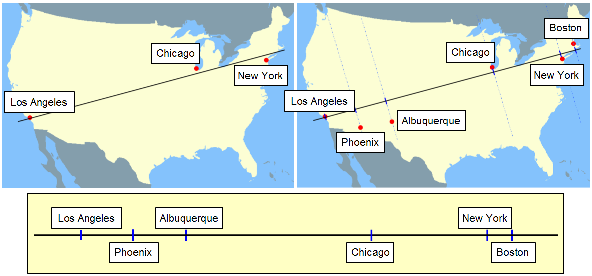
\includegraphics[height=9.5cm,width=12.5cm]{figuras/2.FundamentacaoTeorica/PCAexemploMapa.png}
		\end{center}
		\caption{Mapa exemplo para redução de dimensionalidade \cite{hewitt}.}
		\label{exemploPCA}
	\end{figure}

Embora a linha encontrada acima seja um objeto 1D, esta é localizada dentro de um espaço maior, 2D, e tem como orientação sua inclinação. A inclinação da linha expressa algo importante sobre os três pontos. Ele indica a direção em que eles estão mais espalhados \cite{hewitt}.

Se posicionarmos a origem do nosso plano cartesiano em algum lugar dessa linha, podemos escrever a equação da linha como uma simples $y = mx$, onde $\displaystyle m$ é a inclinação da linha: $dy / dx$ \cite{hewitt}.

Quando ela é descrito desta maneira, a linha é um subespaço do espaço 2D definido pelo sistema de coordenadas. Esta descrição enfatiza o aspecto dos dados que estamos interessados, ou seja, a direção que mantém esses pontos mais separados um do outro \cite{hewitt}.

Esta direção da separação máxima é chamada de primeira componente principal de um conjunto de dados. A próxima direção com máxima separação é a perpendicular a esta. Essa é a segunda componente principal. Em um conjunto de dados 2D, podemos ter no máximo duas componentes principais \cite{hewitt}.

No entanto, o número de componentes principais que podemos encontrar também é limitada pelo número de pontos de dados. Para ver o porque disto, podemos pensar em um conjunto de dados que consiste de apenas um ponto. Não há sentido da separação máxima para esse conjunto de dados, porque não há nada para separar. Agora, considere um conjunto de dados com apenas dois pontos. A linha que conecta esses dois pontos é a primeira componente principal. Mas não há uma segunda componente principal, porque não há nada mais para separar, pois os dois pontos estão totalmente na linha \cite{hewitt}.

Em \textit{Eigenfaces}, cada imagem da face, de tamanho 50x50, é tratada como um ponto com 2500 dimenções. Portanto, o número de componentes principais que podemos encontrar nunca será maior que o número de imagens de faces menos um \cite{hewitt}.

Embora seja importante ter um entendimento conceitual do que as componentes principais são, você não precisa saber os detalhes de como encontrá-las para implementar o \textit{Eigenface}. Essa parte já foi implementada em bibliotecas de processamento de imagens \textit{open source}, como por exemplo a bliblioteca \textit{OpenCV} \cite{hewitt}.

O processo de encontrar um ponto correspondente num subespaço de menor dimensão se chama projeção. Há uma função no \textit{OpenCV} para projetar os pontos sobre um subespaço, então, novamente, você só precisa de um entendimento conceitual. Você pode deixar os detalhes algorítmicos para a biblioteca \cite{hewitt}.

As marcas azuis na Figura \ref{exemploPCA} mostram as localizações no subespaço das três cidades que definiram a linha. Outros pontos 2D também pode ser projetado para esta linha. O lado direito da Figura \ref{exemploPCA} mostra a localização prevista para Phoenix, Albuquerque, Boston \cite{hewitt}.

Em \textit{Eigenface}, a distância entre duas imagens é a distância euclidiana entre os pontos projetados em um subespaço, ao invés da distância no espaço original da imagem de 2500 dimenções. A distância entre as faces neste subespaço de menor dimensão é a técnica utilizada para melhorar a relação sinal / ruído \cite{hewitt}.

Muitas técnicas avançadas de reconhecimento de face são extensões deste conceito básico. A principal diferença entre \textit{Eigenface} e estas técnicas avançadas é o processo de definição do subespaço. Em vez de usar PCA, o subespaço pode ser baseada em Análise de Componentes Independentes (ICA) ou em Análise Discriminante Linear (LDA), e assim por diante \cite{hewitt}.

Em nossa definição de uma linha como um subespaço 1D, usamos $\displaystyle x$ e $\displaystyle y$ coordenadas para definir $\displaystyle m$, que é sua inclinação em 2D. Quando $\displaystyle m$ é um componente principal de um conjunto de pontos, ela é chamada de autovetor ou \textit{eingenvector}, daí o nome \textit{Eigenface} \cite{hewitt}. 

Para o reconhecimento facial em imagens de 50x50, cada autovetor representa a inclinação de uma linha em um espaço de 2.500 dimenções. Como no caso 2D, precisamos de todas as 2.500 dimensões para definir a inclinação de cada linha. Embora seja impossível visualizar uma linha em muitas dimensões, podemos visualizar os autovetores de uma maneira diferente. Podemos converter as suas 2.500 dimenções em uma simples imagem usando a sua ``inclinação'' para colocar cada pixel valor em seu local correspondente. Quando fazemos isso, obtemos imagens \textit{facelike} chamadas de \textit{Eigenface} \cite{hewitt}.

\textit{Eigenfaces} é um método interessante para dar-nos alguma intuição sobre os componentes principais para o nosso conjunto de dados. O lado esquerdo da Figura \ref{exemploEigenfaces} mostra as imagens das faces de dez pessoas. Estas imagens foram encontradas no \textit{Yale Face Database B} (referências 4 e 5). Ele contém imagens de rostos com uma variedade de condições de iluminação. Foram usadas sete imagens de cada uma dessas dez pessoas para criar um subespaço PCA \cite{hewitt}. 

O lado direito da Figura \ref{exemploEigenfaces} mostra os seis primeiros componentes principais deste conjunto de dados, apresentados como eigenfaces. O \textit{Eigenfaces} muitas vezes têm um olhar fantasmagórico, porque combinam elementos de várias faces. As regiões de pixels mais brilhantes e as regiões mais escuras em cada imagem são as que mais contribuem para as componentes principais \cite{hewitt}. 

	\begin{figure}[hbt]
		\begin{center}
			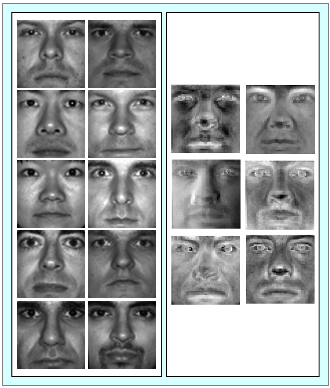
\includegraphics[width=12cm]{figuras/2.FundamentacaoTeorica/eigenfaces.png}
		\end{center}
		\caption{Direita: imagens de rosto para dez pessoas. Esquerda: os seis primeiros componentes principais, visto como \textit{Eigenfaces} \cite{hewitt}.}
		\label{exemploEigenfaces}
	\end{figure}

As componentes principais encontradas pelo PCA apontam para a maior variação de dados. Uma das premissas do \textit{Eigenfaces} é que a variabilidade das imagens subjacentes correspondem à diferença entre as faces. Esta suposição nem sempre é válida. A Figura \ref{exemplosImagensIluminacaoo} mostra as faces de dois indivíduos apresentadas em quatro diferentes condições de iluminação \cite{hewitt}.

Na verdade, elas são imagens de faces de duas das dez pessoas mostradas na Figura \ref{exemploEigenfaces}. Quando a iluminação é muito variável esse algoritmo não é muito efetivo \cite{hewitt}.

	\begin{figure}[hbt]
		\begin{center}
			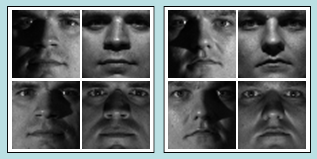
\includegraphics[width=14cm]{figuras/2.FundamentacaoTeorica/exemplosImagensIluminacaoo.png}
		\end{center}
		\caption{Imagens das faces de dois indivíduos. A face de cada indivíduo é apresentada em quatro diferentes cosndições de iluminação. A variabilidade devido à iluminação aqui é maior do que a variabilidade entre os indivíduos. Eigenfaces tende a confundir as pessoas quando os efeitos de iluminação são muito fortes \cite{hewitt}.}
		\label{exemplosImagensIluminacaoo}
	\end{figure}

Outros fatores que podem aumentar a variabilidade da imagem em direções que tendem a diluir a identidade no espaço PCA incluem mudanças na expressão, ângulo da câmera e posição da cabeça \cite{hewitt}.

A Figura \ref{exemploEspacoPCA} mostra como a distribuição de dados afeta o desempenho do Eigenfaces.

Quando os pontos referentes as imagens de cada indivíduo ficam aglutinadas e satisfatoriamente separadas das imagens do conjunto de imagens de outros individuos temos o melhor caso para o funcionamento do Eigenfaces.

Caso os pontos referentes as imagens dos indivíduos tenham uma variabilidade muito grande, a probabilidade de choque de imagens de dois indivíduos num mesmo ponto do subespaço PCA se torna muito grande tornando extremamente difícil separar os dois indivíduos \cite{hewitt}.

Na prática, a projeção de determinadas imagens de uma pessoa no subespaço PCA provavelmente colidirá com projeções de imagens de outras pessoas. Como os autovetores (eigenvector) são determinados pela variabilidade dos dados, ficamos limitados a quão grande deve ser essa. Podemos tomar medidas para limitar, ou para gerir de outra forma, as condições ambientais que podem confundi-lo. Por exemplo, colocar a câmera na altura do rosto irá reduzir a variabilidade no ângulo da câmera \cite{hewitt}.

As condições de iluminação, tais como iluminação lateral vinda de uma janela, são mais difíceis de controlar. Mas você pode considerar o acréscimo de inteligência em cima de reconhecimento facial para compensar isso. Por exemplo, se sabemos onde ele está localizado, e em que direção está olhando, ela pode comparar a imagem do rosto atual apenas com aquelas em situação semelhante \cite{hewitt}.

Mesmo com sistemas altamente ajustados, sistemas de reconhecimento facial estão sujeitos a casos de identidade equivocada \cite{hewitt}.

	\begin{figure}[hbt]
		\begin{center}
			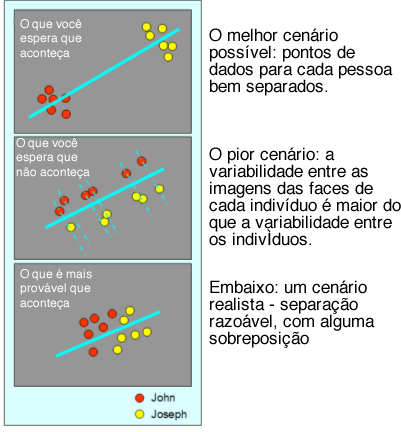
\includegraphics[width=10cm]{figuras/2.FundamentacaoTeorica/espacoPCA.png}
		\end{center}
		\caption{Como as distribuições de dados afetam o reconhecimento com Eigenfaces. Topo: O melhor cenário possível - pontos de dados para cada pessoa bem separados. Meio: O pior cenário - a variabilidade entre as imagens das faces de cada individuo é maior do que a variabilidade entre os indivíduos. Embaixo: um cenário realista - separação razoável, com alguma sobreposição \cite{hewitt}.}
		\label{exemploEspacoPCA}
	\end{figure}


%Como mencionado em cima, essa idéia básica - redução de dimensionalidade seguido pelo cálculo da distância em um subespaço - é amplamente utilizado no trabalho de visão computacional. Também é utilizado em outros ramos da AI. Na verdade, é uma das principais ferramentas para gerenciar a complexidade e para encontrar padrões escondidos dentro de enormes quantidades de dados do mundo real.


